\documentclass[preview,border=7pt]{standalone}
\usepackage{amsmath,amssymb,xcolor}
\usepackage{tikz}
\usetikzlibrary{arrows.meta}
\definecolor{acc}{RGB}{47,143,132}
\definecolor{cyn}{RGB}{6,182,212}
\definecolor{amb}{RGB}{245,158,11}
\begin{document}
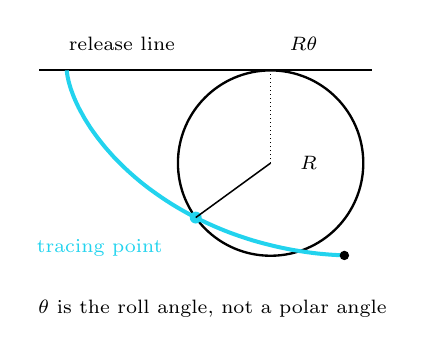
\begin{tikzpicture}
\definecolor{cycol}{RGB}{34,211,238}
\draw[line width=.7pt] (-0.35,0) -- (3.875,0);
\node at (0.70,0.34) {\scriptsize release line};
\draw[line width=.85pt] (2.588,-1.177) circle (1.177);
\draw[cycol, line width=1.45pt] plot[smooth] coordinates {(0.000,0.000) (0.000,-0.000) (0.000,-0.000) (0.000,-0.000) (0.000,-0.000) (0.000,-0.000) (0.000,-0.000) (0.000,-0.000) (0.000,-0.001) (0.000,-0.001) (0.000,-0.001) (0.000,-0.002) (0.000,-0.003) (0.000,-0.004) (0.000,-0.005) (0.000,-0.007) (0.000,-0.009) (0.001,-0.011) (0.001,-0.014) (0.001,-0.018) (0.001,-0.022) (0.002,-0.026) (0.002,-0.032) (0.003,-0.038) (0.004,-0.045) (0.005,-0.052) (0.007,-0.061) (0.008,-0.071) (0.010,-0.082) (0.013,-0.094) (0.016,-0.108) (0.019,-0.123) (0.023,-0.139) (0.028,-0.157) (0.033,-0.176) (0.039,-0.197) (0.046,-0.220) (0.054,-0.245) (0.064,-0.271) (0.074,-0.299) (0.086,-0.330) (0.099,-0.362) (0.114,-0.396) (0.131,-0.433) (0.150,-0.472) (0.171,-0.512) (0.195,-0.555) (0.220,-0.601) (0.249,-0.648) (0.280,-0.697) (0.314,-0.749) (0.352,-0.802) (0.393,-0.858) (0.438,-0.915) (0.486,-0.975) (0.539,-1.035) (0.595,-1.098) (0.656,-1.161) (0.722,-1.226) (0.793,-1.292) (0.869,-1.359) (0.949,-1.426) (1.035,-1.493) (1.127,-1.560) (1.224,-1.627) (1.327,-1.694) (1.435,-1.759) (1.549,-1.823) (1.669,-1.885) (1.795,-1.945) (1.927,-2.003) (2.064,-2.058) (2.207,-2.109) (2.355,-2.157) (2.509,-2.200) (2.668,-2.239) (2.831,-2.273) (2.999,-2.301) (3.171,-2.324) (3.346,-2.340) (3.525,-2.350)};
\fill[cycol] (1.637,-1.869) circle (2.15pt);
\draw[line width=.55pt] (2.588,-1.177) -- (1.637,-1.869);
\draw[line width=.45pt, densely dotted] (2.588,-1.177) -- (2.588,0);
\node at (2.588+0.42,0.34) {\scriptsize $R\theta$};
\node[cycol] at (1.637-1.22,-1.869-0.38) {\scriptsize tracing point};
\node at (2.588+0.48,-1.177) {\scriptsize $R$};
\fill (3.525,-2.350) circle (1.7pt);
\node at (1.85,-3.02) {\scriptsize $\theta$ is the roll angle, not a polar angle};
\end{tikzpicture}
\end{document}
